\documentclass[letterpaper,12pt]{article} % Documento en dos columnas, tamaño carta
\usepackage[spanish]{babel}       % Traduce capítulos, fechas, etc. al español
\usepackage[utf8]{inputenc}       % Permite usar acentos directamente
\usepackage[T1]{fontenc}          % Codificación para que se vean bien los caracteres en PDF
\usepackage{lmodern}              % Usa fuentes escalables compatibles con microtype
\usepackage{geometry}             % Control de márgenes y tamaño de página
\usepackage{fancyhdr}            % Encabezados y pies de página personalizados
\usepackage{background} 

%Notación 

\usepackage{amsmath}  % Ecuaciones, símbolos y fuentes matemáticas
\usepackage{amssymb}
\usepackage{amsfonts}
\usepackage{siunitx}                     % Escritura coherente de unidades del SI y números

%gráficos 

\usepackage{graphicx}           % Insertar y escalar imágenes
\usepackage{subcaption}         % Subfiguras dentro de una figura
\usepackage{booktabs}           % Tablas más profesionales
\usepackage{longtable}          % Tablas que ocupan varias páginas
\usepackage{tabularx}           % Tablas con ancho ajustable automáticamente
\usepackage{array}              % Mejoras en tablas y alineación de columnas
\usepackage{float}              % Control de posición de figuras y tablas


% --- COLORES Y LISTAS PERSONALIZADAS ---
\usepackage{xcolor}             % Uso de colores en texto y figuras
\usepackage{enumitem}           % Listas personalizadas (espaciado, numeración)

% --- HIPERVÍNCULOS Y NAVEGACIÓN ---
\usepackage[hidelinks]{hyperref}           % Enlaces ciclables en PDF (índice, URLs, referencias)
\usepackage{biblatex}           % Gestión de bibliografía (citas, referencias)

% --- DIAGRAMAS TÉCNICOS ---
\usepackage{tikz}                         % Gráficos vectoriales (bloques, flujos, redes)
\usepackage{forest}                      % Árboles, jerarquías (estructuras)

% --- ALGORITMOS Y CÓDIGO FUENTE ---
\usepackage{algorithm2e}    % Pseudocódigo paso a paso (algoritmos)
\usepackage{listings}       % Mostrar código fuente con formato

\geometry{letterpaper, margin=1in} % Márgenes de 1 pul
\title{Ayahuik 1: Guía de Misión}
\author{CUAUHTÉMOC IPN}

\backgroundsetup{
  scale=2,
  color=black,
  opacity=0.05,   % Transparencia
  angle=0,
  position=current page.center,
  contents={\includegraphics[width=0.4\textwidth]{CIPN.jpg}}
}

\pagestyle{fancy} 
\setlength{\headheight}{14.5pt}
\fancyhf{}
\fancyhead[C]{Cuauhtemoc IPN}
\fancyhead[R]{AYAHUIK 1}
\fancyhead[L]{Guia de Misión}
\fancyfoot[R]{\thepage}

\graphicspath{{Imagenes/}}

\begin{document}

\tableofcontents


\newpage
\section{Antecedentes}

    \subsection{Antecedentes Históricos}
    Desde tiempos prehistóricos el hombre se ha percatado de sus propias capacidades físicas y así de sus limitaciones, una de ellas es la de logra el vuelo por medios propios y valiéndose de su propia fortaleza, como es el caso de las aves y algunos mamíferos.
Con base en el principio de Arquímedes utilizado como flotabilidad dentro de un fluido se sabe que un fluido a mayor temperatura tiene menor densidad o un gas menos denso del que lo envuelve tendera a desplazarse hacia arriba. 
Así se demostró en agosto de 1709, ya que el sacerdote brasileño Bartolomeu de Gusmão hizo la primera demostración de ascensión aérea en globo de aire caliente no tripulado en la Casa de Indias de Lisboa, ante la corte del rey Juan V de Portugal .

\begin{figure}[H]
      \centerline{\includegraphics[width=.6\textwidth]{BG-0000.jpg}}
      \caption{Modelo de Bartolomeu de Gusmão}
      \label{fig:BG}
\end{figure}
Posteriormente Joseph y Jacques Montgolfier lanzaron su primer modelo en septiembre de 1782. El 4 de junio de 1783 realizaron una demostración pública con un globo aerostático de diez metros de diámetro, construido con tela y papel .
En México se refiere , que en Xalapa, Veracruz, fue José María Alfaro quien logró elevar un globo aerostático de aire caliente y de cubierta impermeable en 1784. Casi un año más tarde, el 6 de febrero de 1785, el militar Antonio María Fernández elevó un globo más pequeño, en el Puerto de Veracruz.  Durante 1785 hubo varios otros vuelos en Veracruz (algunos sucesos fueron "prósperos" y otros "adversos").
En años más recientes , a finales  del Siglo XIX,  se puso de moda el volar y asistir a funciones de globos aerostáticos como pasatiempo. En México,  varios expertos aeronautas internacionales habían ofrecido algunas demostraciones de vuelo en la capital del país,  pero tuvieron poco éxito.

\begin{figure}[H]
      \centerline{\includegraphics[width=.4\textwidth]{jma.jpeg}}
      \caption{Representación vuelo Jose Maria Alfaro}
      \label{fig:JMA}
    \end{figure}

Joaquín De la Cantolla , inspirado por los globos de los hermanos Montgolfier y el vuelo del guanajuatense Benito León Acosta en 1844, fundó la Empresa Aerostática de México y en el año 1862 solicitó apoyo del gobierno para realizar ensayos personales sobre aerostatos de dirección.
El 26 de junio de 1863, él anunció una ascensión en, que tuvo lugar en la Plaza de Toros del Paseo Nuevo. 
El éxito de la experiencia convertiría a sus globos en un elemento básico de las fiestas populares de México, bien para asombro bien para diversión. 
Los globos de De la Cantolla eran de manta inglesa cortada y cosida. De la Cantolla inventó un sistema regulador de la llama de alcohol para graduar el ascenso y el descenso del globo para mejora la alimentación con aire caliente. El invento fue analizado por expertos y probado con éxito el 22 de octubre de 1877 en el patio de la Escuela de Ingenieros del Colegio de Minería. 
De la Cantolla construyó varios globos para sus paseos por México, el Moctezuma I
Moctezuma II, Construido tras el éxito de Moctezuma 1, los retales eran blancos, verdes y rojos como la bandera mexicana. Tenía un tamaño similar. Este es el globo que se representó en el mural "La conquista del aire por el hombre" de Juan O'Gorman, en el Aeropuerto Internacional de la Ciudad de México. En este mural aparece la frase "Viva Cantoya".
Vulcano. El globo más grande se llamaba “Vulcano”. Hinchado medía unos 20 metros. A mitad de la tela tenía un adorno de tela roja con flecos dorados y cuatro águilas imperiales pintadas
Globos de Cantolla. En algún momento de su vida, diseñó globos construyéndolos de pequeño tamaño con papel. Estos globos se soltaban por cientos en fiestas populares, son de un tamaño muy pequeño sin la posibilidad de ser tripulados.

\newpage
    \subsection{Antecedentes ESIME TICOMAN}

    La carrera de Ingeniería en Aeronáutica comenzó a impartirse dentro del Instituto Politécnico Nacional en el año de 1937; a lo largo de los 79 años de existencia ha dado soporte a todas las actividades de nuestro país en los ámbitos de Diseño, Construcción y Operación de la Aeronaves que se han construido en México y a los proyectos espaciales en los que se ha participado . Cabe hacer mención que hasta el año 2007 fue la única escuela a nivel nacional que impartía la carrera de Ingeniaría en Aeronáutica.

    \begin{figure}[H]
      \centerline{\includegraphics[width=.3\textwidth]{ESIME.png}}
      \caption{LOGO ESIME TICOMAN}
      \label{fig:ESIME2}
    \end{figure}
A partir del año 2012 se comienza a impartir la Maestría en Ciencias de la Ingeniería Aeronáutica y Espacial, en la cual una de sus líneas de investigación es “Tecnología Espacial y Percepción Remota”, dentro de la cual se estudian la tecnología de Satélites y  cohetes lanzadores.
Se han tenido intercambios de estudiantes y profesores con el Instituto de Aviación de Moscú, la Universidad Nacional Aeroespacial de Ucrania, el Centro de Investigación Ames de la NASA, la Universidad Técnica de Múnich, la Universidad Politécnica de Madrid, La Escuela Nacional Superior de Aeronáutica y el Espacio (ENSAE, Sup’Aero) de Francia, entre muchas otras.
Durante el proyecto Multinstitucional del Microsatélite Satex 1, propuesto por el Instituto Mexicano de Comunicaciones en 1994, la ESIME Ticomán fue la responsable del diseño y construcción de la estructura de Vuelo, el ensamble la integración y las pruebas del satélite, construyéndose dentro de sus instalaciones una sala de integración compuesta por un cuarto limpio clase 10,000 dotado con una campana de flujo laminar clase 1000 y un área de usos múltiples. 

\begin{figure}[H]
      \centerline{\includegraphics[width=.3\textwidth]{satex.jpeg}}
      \caption{SATEX 1}
      \label{fig:satex}
\end{figure}

Este proyecto no fue concluido debido a la falta de fondos; sin embargo, todas las instituciones desarrollaron las capacidades requeridas para desarrollar el proyecto. Destacando que ESIME Ticomán termino las actividades comprometidas y ha quedado la infraestructura disponible para nuevos proyectos.
Diversos egresados y profesores de la ESIME Ticomán participaron en los proyectos de la Comisión Nacional del Espacio Exterior, trabajaron dentro de programa de satélites Morelos y Solidaridad, al crearse la empresa SATMEX, miembros de esta comunidad trabajaron de forma fija y en proyectos espaciales, y en el programa MEXSAT, de igual manera han contribuido en el seguimiento al proceso de pruebas del satélite y participando en las negociaciones para su lanzamiento, puesta en órbita y operación.
Durante el 2013 se participó en conjunto con el Centro de Investigación Ames de la NASA, la Universidad Autónoma de Baja California y la Universidad de California en San José en el desarrollo del proyecto AztechSat 1, para el diseño y construcción de un nanosatélite dentro del estándar cubesat de una unidad, concluyendo satisfactoriamente la Revisión Crítica del Diseño y la interconexión de todos los sistemas (FlatSat).
Actualmente, se participa como responsable del Diseño Estructural, Ensamble, Integración y Pruebas de dos nanosatélites bajo el estándar cubesat de tres unidades, para un cliente privado que ha solicitado la confidencialidad hasta el fin del proyecto. Un prototipo del proyecto se encuentra ya en la fase de pruebas.
Laboratorio de Integración y Pruebas AeroEspaciales (LIPAE) de ESIME Ticomán. Equipamiento actual, con la infraestructura creada para el proyecto SATEX 1 , y con la adquisición y puesta en marcha de una mesa de Vibraciones Mecánicas  en tres ejes y capacidad de vibrar desde 4 hasta 4,000 Hz, masas de hasta 50 Kg. Sala gris de 110 mts.

\begin{figure}[H]
      \centerline{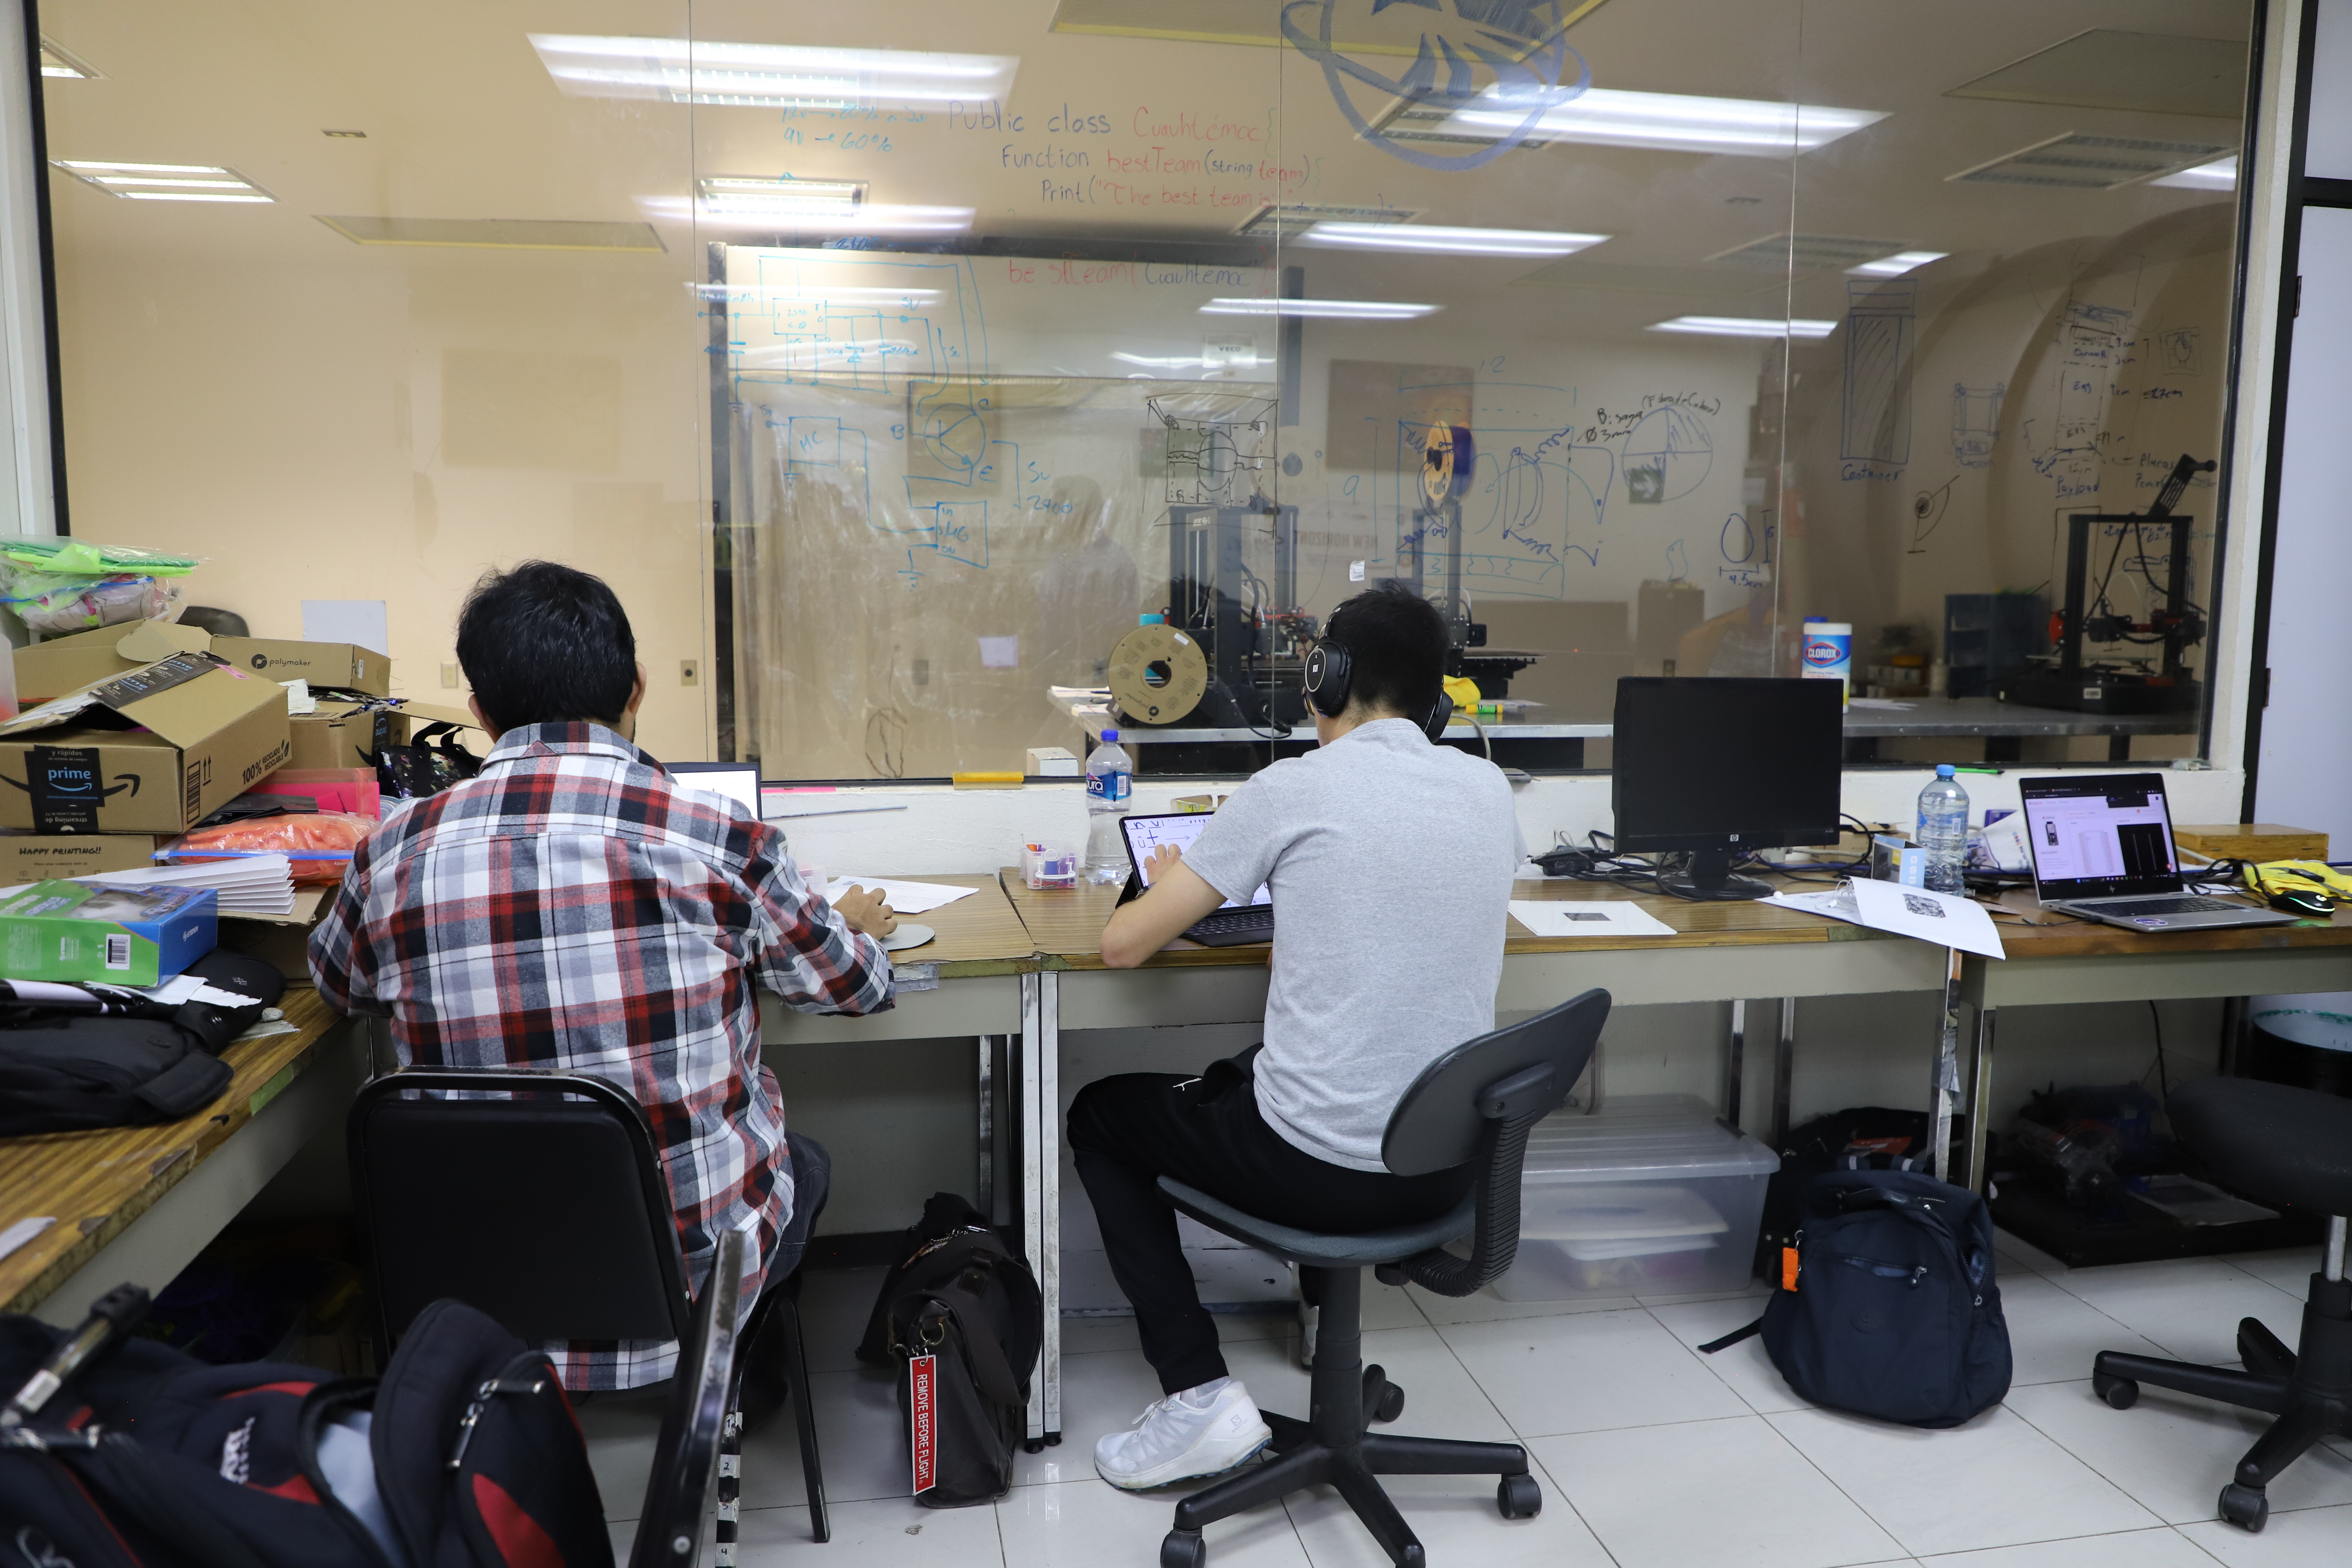
\includegraphics[width=.5\textwidth]{lab.jpg}}
      \caption{LIPAE}
      \label{fig:LAB}
    \end{figure}

\newpage
    \subsection{Antecedentes Cuauhtémoc IPN}

    El equipo CUAUHTÉMOC IPN al momento de la realización de esta misión cuenta con una trayectoria de 9 años en la 
    participación de misiones tanto nacionales como internacionales, con su primera participación en la misión CANSAT Competition 
    2017 y CANSAT CUCEI 2017, en las cuales se obtuvieron 5to lugar internacional y 2do lugar nacional respectivamente, en este tiempo
    a partir de su fundación el equipo a tenido participación en mas de 14 misiones de las cuales hemos obtenido reconocimiento nacional e 
    internacional.
    
    \begin{figure}[H]
      \centerline{\includegraphics[width=.6\textwidth]{CUAUH.jpg}}
      \caption{CUAUHTÉMOC IPN CANSAT Competition 2017}
      \label{fig:CC2017}
    \end{figure}

    A lo largo de toda esta trayectoria hemos obtenido experiencia en el desarrollo de demostradores tecnológicos como CANSAT, Rovers autónomos
    y picosatelites, cada uno con una misión completamente diferente a la anterior lo cual nos ha hecho tener experiencia en una gran variedad de ámbitos, 
    siempre a la vanguardia y con la vision de superarnos en retos cada dia.
    
    \begin{figure}[H]
      \centerline{\includegraphics[width=.6\textwidth]{cipn2.jpg}}
      \caption{CUAUHTÉMOC IPN CANSAT Competition 2024}
      \label{fig:CC2024}
    \end{figure}

    \newpage

    Tanto para las competencias nacionales como las internacionales todos los modelos son desarrollados íntegramente por el equipo, desde el area electronica 
    , el area mecánica, hasta el area aerodinámica, siendo todo diseñado y manufacturado por jóvenes estudiantes de multiples unidades académicas del IPN.
    Todos los modelos y manufactura se llevan a cabo dentro del laboratorio de integración y pruebas aeroespaciales de la ESIME Unidad Ticoman del IPN.

    \begin{figure}[H]
      \centerline{\includegraphics[width=.5\textwidth]{cipn3.jpg}}
      \caption{Desarrollo CUCEI 2017}
      \label{fig:DC}
    \end{figure}

    \newpage

\section{Descripción general de la misión}

    \subsection{Participantes de la misión}

    La misión Ayahuik 1 es una misión de alto impacto del equipo Cuauhtémoc IPN, la cual tendrá
    participación de varios estudiantes de diferentes unidades académicas del IPN, incluidas ESIME Ticoman, 
    ESIME Culhuacan, ESIME Zacatenco, UPIITA, ESCOM, ESIQUIE entre otras, asi como profesores asesores de las mismas 
    unidades académicas.

    \subsection{CONOPS}

    A partir de de las simulaciones con las fechas y horas establecidas se procederá a:

    \medskip   \qquad Se llenara el globo de helio hasta superar su punto de flotabilidad neutra.

    \medskip   \qquad Se iniciaran los sistemas de la carga util.

    \medskip   \qquad Se iniciara la cuenta regresiva para la liberación del globo.
    
    \vspace{5mm}

    Se liberara el globo sonda y se iniciara el vuelo.

    \medskip   \qquad Se iniciara la recolección de datos de telemetria.

    \medskip   \qquad Se deberá realizar monitoreo constante del vuelo.

    \medskip   \qquad Una vez alcanza la altitud objetivo se deberá reventar el globo sonda.

    \medskip   \qquad Se deberá realizar el rastreo contante en el descenso.
    
    \vspace{5mm}

    Una vez que la carga util toque tierra se deberá proceder a su recuperación.

    \medskip   \qquad Se deberá proceder a la recuperación de la carga util.

    \medskip   \qquad Se deberá asegurar tanto cámaras como datos almacenados.

    \subsection{Descripción de la carga util}

    La carga util deberá esta constituida por una plataforma en la cual deberá tener 
    la capacidad de resistir las condiciones adversas de la estratosfera, asi como la obtención
    de los siguientes datos:

    \begin{itemize}
        \item Temperatura, humedad, altitud, aptitud, velocidad, rayos ultravioleta.
        \item Gases atmosféricos (Oxigeno, hidrógeno, nitrógeno).
        \item Gases volcánicos (Dióxido de carbono, Dióxido de azufre).
        \item Posicionamiento GNSS.
        \item Estación meteorológica.
        \item Radio baliza.
        \item Radio localizador.
        \item Cámaras de video y fotografía.
        \item ETC. 
    \end{itemize}

    \subsection{Descripción del proceso de diseño y construcción}

    La metodología de desarrollo para la misión Ayahuik se basa en la utilizada por el equipo Cuauhtémoc IPN a lo largo de su historia
    la cual se basa en una adaptación simplificada y adaptada del NASA Systems Engineering Handbook, dividiendo en 5 etapas el desarrollo de
    la misión las cuales son: 
    
    \subsubsection{Fase de formulación}
        En esta fase se definen los objetivos generales y específicos de la misión, asi como sus limitaciones 
        y criterios de éxito asi como la conformación de los miembros de la misión.

    \subsubsection{Preliminar Desing}

        Se empieza con la fase de investigación técnica asi como el desarrollo
        de conceptos, inicia el desarrollo conceptual de la plataforma y carga util de la misión, asi como los primeros diseños 
        preliminares de la misma.    

    \subsubsection{Critical Design}

        Se concretan los diseños de la plataforma y carga util, siendo que a partir de este momento los cambios realizados antes del 
        lanzamiento deben ser mínimos y justificados por el equipo, se deberán empezar a hacer pruebas de funcionamiento y la integración del 
        modelo de ingeniería para probar todos los sistemas trabajando en conjunto.

    \subsubsection{Pruebas ambientales}

        Se deberán realizar 4 pruebas ambientales para verificar el correcto funcionamiento de todos los sistemas y mecanismos de la plataforma 
        asi como verificar el desempeño estructural de la misma, estas pruebas son descritas a continuación:

        \subsubsection*{Termal Test}
        Esta prueba consiste en llevar a la plataforma a temperaturas elevadas (60C $\pm$ 5C ) para validad el correcto funcionamiento de los sistemas en 
        condiciones atmosféricas adversas, asi como para validad los sistemas de medición de temperatura a bordo.

        \subsubsection*{Vacuum Test}
        
        Bajando la presión abruptamente del modelo en una cámara sellada se comprueba el funcionamiento de los sistemas de medición de presión externa
        asi como para validar los sistemas abordo los cuales dependen de la presión atmosférica externa como altitud y etapas de la misión asi como los mecanismos dependientes
        de los mismos.

        \subsubsection*{Vibration Test}

        Para validar el correcto ensamblaje del modelo este se ve sujeto a un proceso en el cual es sometido a diferentes vibraciones en diferentes frecuencias y amplitudes, midiendo 
        constantemente las variaciones en el comportamiento estructural del modelo para verificar que no halla cambios estructurales abruptos en la misión.
        
        \subsubsection*{Drop Test}

        El modelo es sometido a una gran cantidad de Gs para poder validar su resistencia a impactos asi como la integridad estructural de la estructura, esto certifica que el modelo 
        no sufrirá daños al momento del despliegue del paracaídas y aterrizaje.

    \subsubsection{Lanzamiento y misión}

    En le fecha y horas establecidas se llevara a cabo el lanzamiento de la misión, en las cuales de deberá evaluar el porcentaje de cumplimiento de los objetivos y metas del proyecto,
    asi como la recopilación de los datos establecidos y recuperación al momento del descenso.

    \subsubsection{Post Flight}

    Posterior a la conclusion de la etapa de vuelo se deberá llevar a cabo el procesamiento final de los datos obtenidos asi como una retroalimentación tanto técnica como general de los logros y conocimientos adquiridos durante la misión que fungirán como memoria histórica, finalmente se deberá llevar a cabo una evaluación 
    de todas las etapas de la misma, dando asi finalización a la misión AYAHUIK 1.



    \subsection{Descripción del lanzamiento y recuperación}

    Al momento del lanzamiento del globo sonda, este deberá contar con análisis previos
    de trayectoria ya que la cuenca del valle de Mexico y las zonas cercanas contienen rutas
    aéreas de gran importancia del país asi como la cercanía de varios aeropuertos los cuales 
    son el aeropuerto Marino Matamoros, aeropuerto Internacional de Toluca, Aeropuerto internacional de Prueba, Aeropuerto Nacional Mexiquense “Dr. Jorge Jiménez Cantú”
    y el mas importante el Aeropuerto Internacional de la Ciudad de México el cual es el
    mas importante del país, por lo cual se debe contar con un plan de vuelo y una trayectoria 
    que evite zonas restringidas nacionales e internacionales, así como evitar rutas aéreas de gran importancia.
    Por lo mismo se deberá contar con los permisos necesarios por parte de la Dirección General de Aeronáutica Civil,
    Agencia Federal de Aviación Civil para el lanzamiento del globo sonda.

    \begin{figure}[H]
      \centerline{\includegraphics[width=1\textwidth]{Tray.png}}
      \caption{Trayectorias estimadas para el mes de Julio}
      \label{fig:Trayectoria}
    \end{figure}

    \begin{figure}[H]
      \centerline{\includegraphics[width=.8\textwidth]{Zonas.png}}
      \caption{Zonas con restricciones aéreas cercanas}
      \label{fig:Zonas}
    \end{figure}

    \begin{figure}[H]
      \centerline{\includegraphics[width=.8\textwidth]{Espacioaereo.png}}
      \caption{Espacio y transito aéreo sobre el valle de la ciudad de Mexico}
      \label{fig:Espacio}
    \end{figure}

    Se deberá realizar un análisis exhaustivo en conjunto de las autoridades mexicanas 
    para decidir el mejor dia y hora del lanzamiento del globo sonda, la zona de recuperación se 
    establecerá en varios puntos a partir de las simulaciones de trayectoria y el viento, asi como 
    la trayectoria qeu siga el globo al momento del vuelo.


\newpage
\section{Objetivos y criterios de éxito}

    \subsection{Objetivos generales}
    La misión Ayahuik 1 tiene como objetivo principal el desarrollo de una carga util capaz de ser lanzada a la estratosfera
    y recuperar parámetros atmosféricos y de condiciones del aire a diferentes alturas,
    así como la obtención de material fotográfico y de video del lanzamiento y vuelo de la misma.


    Esto con el fin de la obtención de datos científicos como de divulgación.

    \subsection{Objetivos específicos}
    \begin{itemize}
        \item El desarrollo de una carga util de un globo sonda la cual demuestre las capacidades desarrollo tecnológico de los miembros del equipo Cuauhtémoc IPN.
        \item Fotografía y video de las zonas aledañas al volcán Popocatepetl.
        \item Sondeo de gases en diferentes altitudes en las zonas aledañas al volcán Popocatepetl.
        \item Recolección de datos atmosféricos y de condiciones del aire a diferentes alturas
        \item Capacitación de las nuevas generaciones del equipo tanto en ámbitos tecnológicos como de documentación y divulgación.
        \item Incentivación del desarrollo de nuevas tecnologías y retos para los miembros del equipo.
        \item Divulgación científica con los datos y videos obtenidos al vuelo.
        
    \end{itemize}    

    \newpage
    
    \subsection{Criterios de éxito}

    Los criterios de éxito de la misión se basaran en una ponderación al 100\% de los hitos obtenidos durante el desarrollo de la misión en su etapa de vuelo dependiendo de su importancia y complejidad los cuales son desarrollados a continuación:

    \begin{longtable}{|m{4.1cm}|c|c|c|}
    \hline
    \textbf{Criterio de Éxito} & \textbf{Puntos máximos} & \textbf{Puntos Obtenidos} & \textbf{Observaciones} \\
    \hline
    \endfirsthead
    \hline
    \textbf{Criterio de Éxito} & \textbf{Puntos máximos} & \textbf{Puntos Obtenidos} & \textbf{Observaciones} \\
    \hline
    \endhead
    Vuelo a grandes altitudes & 50 &  & \\
    \midrule
    Medición de temperatura en vuelo & 40 &  & \\
    \midrule
    Medición de la presión en vuelo & 40 &  & \\
    \midrule
    Medición de oxigeno en vuelo & 20 &  & \\
    \midrule
    Medición de vapor de agua en vuelo & 20 &  & \\
    \midrule
    Medición del gas $H_{2}$ en vuelo & 20 &  & \\
    \midrule
    Medición del gas $CO_{2}$ en vuelo & 20 &  & \\
    \midrule
    Medición del gas $SO_{2}$ en vuelo & 20 &  & \\
    \midrule
    Toma de fotografía del Popocatepetl & 30 &  & \\
    \midrule
    Toma de video del Popocatepetl & 15 &  & \\
    \midrule
    Toma de fotografía del horizonte & 20 &  & \\
    \midrule
    Toma de video del horizonte & 10 &  & \\
    \midrule
    Recepción de telemetria por RF & 50 &  & \\
    \midrule
    Recepción de telemetria por SMS & 40 &  & \\
    \midrule
    Recepción de telemetria por MSM & 40 &  & \\
    \midrule
    Señal GNSS constante & 50 &  & \\
    \midrule
    Recuperación total de la carga util & 50 &  & \\
    \midrule
    Estado de la carga util al recuperar & 30 &  & \\
    \midrule
    Control autónomo en la etapa de descenso & 50 & & \\
    \midrule
    Funcionamiento de la Estación Terrena & 50 &  & \\
    \midrule
    Funcionamiento de la computadora de vuelo & 50 &  & \\
    \midrule
    Funcionamiento de la electronica & 50 &  & \\
    \midrule
    \textbf{TOTAL} & 765 &  & -\\
    \hline
    \end{longtable}

    Por lo tanto el porcentaje de Éxito de la misión es de: $\%$

    Éxito mínimo < 50\%

    Éxito parcial 50\% - 80\%

    Éxito total 80\% - 100\%

    \newpage

    \subsection{Restricciones y requerimientos}

    \begin{longtable}{|l|m{15cm}|}
    \hline
    \textbf{No.} & \textbf{Restricción/Requerimiento} \\
    \hline
    \endfirsthead
    \hline
    \textbf{No.} & \textbf{Restricción/Requerimiento} \\
    \hline
    \endhead
    1 & La masa total de la carga útil no debe exceder 1 kg. \\
    \midrule
    2 & La carga util debe ser capaz de soportar las adversas condiciones de 20 km de altitud. \\
    \midrule
    3 & Se debe contar con una reserva energética de al menos el $100\%$ de la misión. \\
    \midrule
    4 & Ningún elemento debe sobresalir del area delimitada para la carga util. \\
    \midrule
    5 & La carga util deberá ser capaz de decender al momento del toque de tierra a 5 m/s verticales. \\
    \midrule
    6 & La carga util deberá estar hecha de colores fosforescentes o reflectantes para su localización. \\
    \midrule
    7 & No se debe usar pirotecnia. \\
    \midrule
    8 & Se debe logar la recolección de todos los datos de vuelo. \\
    \midrule
    9 & Se debe contar con un sistema de GNSS o a través de triangulación por RF. \\
    \midrule
    10 & La telemetria se debe almacenar en una memoria interna. \\
    \midrule
    11 & La telemetria debe ser expuesta en uns estación terrena.   \\
    \midrule
    12 & La telemetria también debe ser enviada por SMS Y MSM. \\
    \midrule
    13 & La carga util debe estar identificada con el nombre del equipo asi como un medio de contacto. \\
    \midrule
    14 & Debe haber un interruptor de apagado y encendido del modelo. \\
    \midrule
    15 & Se debe contar con un sistema de audio beacon para la localización en tierra. \\
    \midrule
    16 & Se debe contar con al menos 2 sistemas de explosion o liberación de emergencia del globo.    \\
    \midrule
    17 & Se debe contar con una radiobaliza \\
    \hline
        
    \end{longtable}

    \newpage
\section{Resultados esperados}

    La misión contara con diferentes resultados esperados, los cuales se dividen en resultados técnicos, de la carga util y de la misión en general, 
    los cuales validaran el correcto desarrollo y éxito total o parcial de la misión.

    \subsection{Resultados técnicos}

    documentación técnica de la carga util y sistemas asi como del desarrollo de los mismos
    (PDR, CDR y PFR).
    Asimismo un documento con los resultados de las pruebas ambientales realizadas (vació, térmica, vibraciones y drop test)
    detallando el desempeño de la carga util y validando a la misma para su lanzamiento. 

    \subsection{Resultados de la carga útil}

    Carga util reutilizable que cumpla con todos los requisitos establecidos para la misión, la cual
    demuestre tener capacidades de recolección de datos y transmisión de los mismos tanto por radio
    frecuencia como por SMS y MSM a una estación terrena.
    
    Esta deberá contar con manual de operaciones 
    para la correcta operación y recuperación de la carga util.
    
    La misma deberá ser capaz de resistir las condiciones de lanzamiento y vuelo con condiciones extremas de presión y temperatura,
    asi como de ser capaz de soportar el retorno a tierra y ser recuperada en condiciones de operatividad.


    \subsection{Resultados de la misión}

    Obtención de datos atmosféricos y de condiciones del aire a diferentes alturas de gran utilidad
    científica y de investigación, asi como material fotográfico y de video del lanzamiento y vuelo desde la carga util.
    
    Aprendizaje y capacitación practica para la nueva generación del equipo Cuauhtémoc IPN 2025-2026 a lo largo de diferentes
    ámbitos tanto de desarrollo técnico como de generación de documentación técnica y de gestión de proyectos de alto impacto. 



\newpage

\section{Organización del equipo}

    El equipo Cuauhtémoc IPN está organizado en diferentes subsecciones para asegurar el funcionamiento del equipo y una gestión 
    eficiente de las misión, todas estas serán coordinadas por los líderes de misión 
    y estos a su ves por los capitanes del equipo. 
    \begin{figure}[!h]
      \centerline{\includegraphics[width=.8\textwidth]{ORG-AYA1-GM-V3.png}}
      \caption{Organigrama Ayahuik 1}
      \label{1}
    \end{figure}
    
    Para la misión Ayahuik 1, el equipo Cuauhtémoc IPN contara con las 2 capitanas del equipo, 
    las cuales se encargaran de coordinar las actividades generales del equipo asi como sus misiones activas, 
    estas son:

    \begin{itemize}
        \item \textbf{Capitana:} Sofia Rojas
        \item \textbf{Subcapitana:} Tania Olmos
    
    \end{itemize}

    De esto se derivara el asesor técnico el cual se encargara de todo el asesoramiento tanto para el funcionamiento del equipo
    como para la correcta realización de la misión sin que este tenga intervención directa, el cual es:

    \begin{itemize}
        \item \textbf{Asesor técnico:} Hector Diaz

    \end{itemize}


    \vspace{5mm}

    El liderato de la misión AYAHUIK 1 estará a cargo de 3 co-líderes,
    los cuales se encargaran de coordinar el correcto funcionamiento de Cada
    una de las subsecciones del equipo, estos son:

    \begin{itemize}
        \item \textbf{Líder administrativo:} Luis Romero
        \item \textbf{Líder técnico:} Andrea Garcia
        \item \textbf{Líder de convergencia:} Brandon Garcia
    
    \end{itemize}

    \subsection{Subsecciones}
    De los 3 co-lideres de la misión se derivan las subsecciones principales del equipo las cuales son:
    
    \subsection*{Aeroestructuras}

    Subsección encargada de todo lo que refiere al area estructural y aerodinámica, desarrolla la estructura y elementos aerodinámicos tanto activos como pasivos.
    
    \subsection*{EPS (Electrical Power System)}

    Encargada de cálculos y diseño de sistemas de potencia que darán vida a todos y cada uno de los sensores y actuadores del CANSAT para su correcto funcionamiento a lo largo de la misión; además del diseño de los circuitos impresos que lleva cada uno de los modelos.
    
    \subsection*{GS (Ground Station)}

    Encargada del desarrollo de software de telemetria análisis y procesamiento de datos de telemetria, así como también los sistemas de comunicación remota.
    
    \subsection*{CDH (Communication and Data Handling)}

    Es la sección encargada del diseño e implementación de sistemas de comunicaciones, así como la programación de sensores y microcontroladores.

    \newpage

\section{Bibliografía}
    \begin{thebibliography}{9}
        \bibitem{NASA} NASA. (2023). High Altitude Ballooning. Recuperado de \url{https://www.nasa.gov/ballooning}
        \bibitem{ESA} ESA. (2023). Stratospheric Balloon Missions. Recuperado de \url{https://www.esa.int/stratospheric_ballooning}
        \bibitem{IPN} Instituto Politécnico Nacional. (2023). Cuauhtémoc IPN. Recuperado de \url{https://cuauhtemoc.ipn.mx}
        \bibitem{ESIME} ESIME Ticoman. (2023). Proyectos de investigación y desarrollo tecnológico. Recuperado de \url{https://esime-ticoman.ipn.mx/proyectos}

    \end{thebibliography}

    \newpage

    \section{Patrocinadores}
    \captionsetup[subfigure]{labelformat=empty}

    \begin{figure}[h!]
    \centering
    \begin{subfigure}[b]{0.3\textwidth}
        \centering
        \includegraphics[height=3cm]{IPN.png}
        \caption{IPN}
        \label{fig:IPN}
    \end{subfigure}
    \hfill
    \begin{subfigure}[b]{0.3\textwidth}
        \centering
        \includegraphics[height=3cm]{ESIME.png}
        \caption{ESIME Ticoman}
        \label{fig:ESIME}
    \end{subfigure}
    \hfill
    \begin{subfigure}[b]{0.3\textwidth}
        \centering
        \includegraphics[height=1.8cm]{FUNDPOL.png}
        \vspace{0.5cm}
        \caption{Fundación Politécnico}
        \label{fig:FUNDPOL}
    \end{subfigure}
    \end{figure}


    \begin{figure}[h!]
    \centering
    \begin{subfigure}[b]{0.3\textwidth}
        \centering
        \includegraphics[height=2cm]{ALTIUM.png}
        \caption{ALTIUM}
        \label{fig:ALTIUM}
    \end{subfigure}
    \hfill
    \begin{subfigure}[b]{0.3\textwidth}
        \centering
        \includegraphics[height=1cm]{ALTAIR.png}
        \vspace{0.1cm}
        \caption{ALTAIR}
        \label{fig:ALTAIR}
    \end{subfigure}
    \hfill
    \begin{subfigure}[b]{0.3\textwidth}
        \centering
        \includegraphics[height=1.2cm]{PCBMEX.png}
        \vspace{0.5cm}
        \caption{PCB México}
        \label{fig:PCBMEX}
    \end{subfigure}
    \end{figure}

    \hspace{0.3cm}
    \begin{figure}[h!]
    \centering
    \begin{subfigure}[b]{0.3\textwidth}
        \centering
        \includegraphics[height=1.1cm]{SSC.png}
        \vspace{0.2cm}
        \caption{GRUPO SSC}
        \label{fig:SSC}
    \end{subfigure}
    \hfill
    \begin{subfigure}[b]{0.3\textwidth}
        \centering
        \includegraphics[height=1.5cm]{ANSYS.png}
        \caption{ANSYS}
        \label{fig:ANSYS}
    \end{subfigure}
    \hfill
    \begin{subfigure}[b]{0.3\textwidth}
        \centering
        \includegraphics[height=1.2cm]{DASSAULT.png}
        \vspace{0.2cm}
        \caption{DASSAULT SYSTEMES}
        \label{fig:DASSAULT}
    \end{subfigure}
    \end{figure}
    
    \hfill


    Gracias por su apoyo, sin ustedes nada de esto sería posible.

    Atte. Cuauhtémoc IPN

    \end{document}
